\chapter{Méthodologie du travail}
\section{Gestion du projet}
Pour notre projet nous avons adopté un processus de développement en spirale cela se manifeste dans la réalisation par exemple des tests unitaires en parallèle lors de la terminaison de chaque module ou package.

\begin{figure}[!h]
\begin{center}
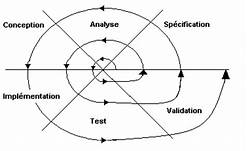
\includegraphics[width=7cm]{proc.png}
\caption{Processus de développement}
\end{center}
\end{figure}
\section{Collaboration}
Comme ce travail a été élaboré par quatre personnes, l'organisation et la synchronisation est une chose primordiale entre nous, dans ce sens, nous avions utilises les deux outils Git et GitHub, en travaillant sur un remote repository, tout en utilisant l'onglet "Projet" dans GitHub,chose qui a facilite l'organisation des taches, comme le montre la figure suivante:
\begin{figure}[!h]
\begin{center}
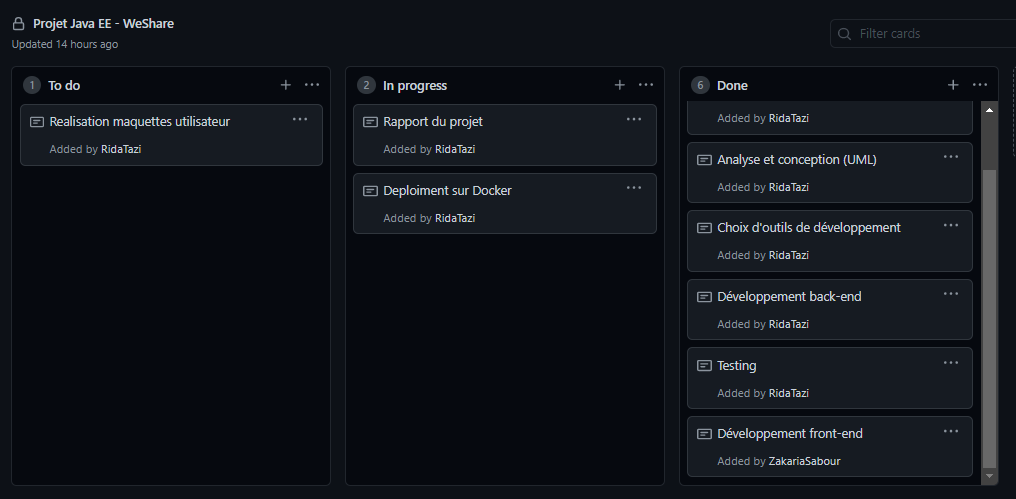
\includegraphics[width=10cm]{projethub.png}
\caption{Projet GitHub}
\end{center}
\end{figure}

Nous avons aussi utilisé MS Teams comme plat-forme de communication, pour assurer des meetings deux a trois fois par semaine.

\chapter{Analyse et conception}
Cette partie présente, en premier lieu, la modélisation
fonctionnelle avec les diagrammes UML.
En second lieu, il définit la conception du projet.
\section{Analyse}
\subsection{Diagramme de cas d'utilisation}
Pour l'analyse, nous avions utilisé le diagramme des cas d'utilisation, avec l'outil PlainUML. En effet, ce diagramme permet la représentation du comportement fonctionnel de notre système, indépendamment du type de l'utilisateur en question.


\begin{figure}[!h]
\begin{center}
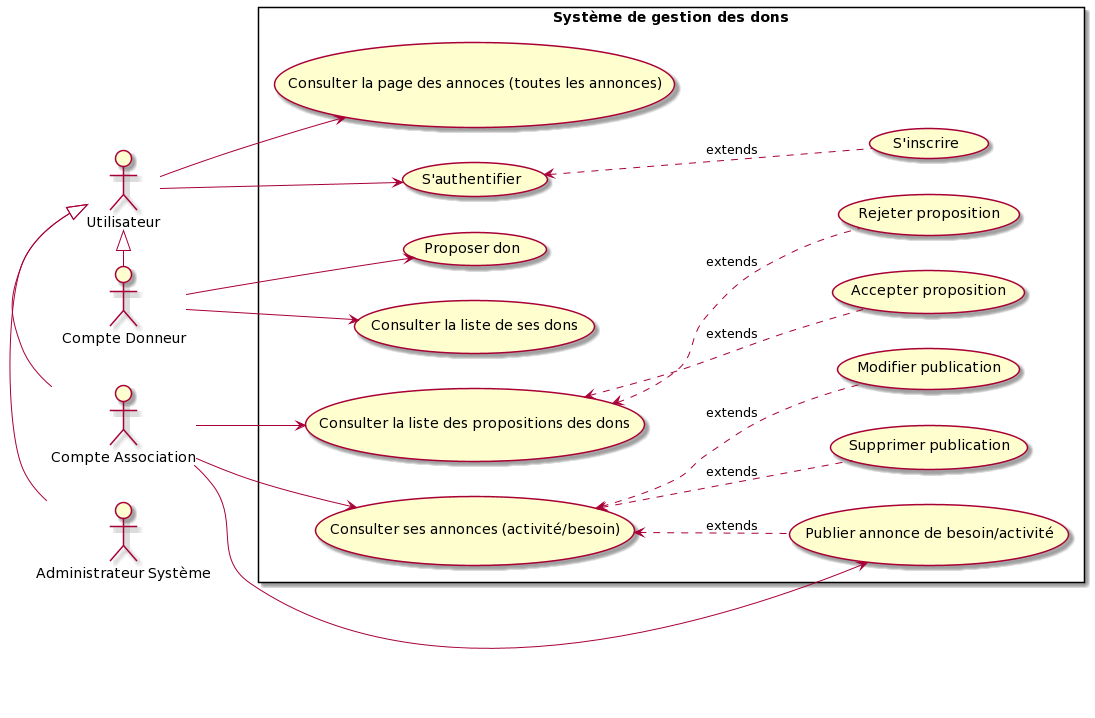
\includegraphics[width=17cm]{DCU.png}
\caption{Diagramme de cas d’utilisation}
\end{center}
\end{figure}

\subsection{Les besoins fonctionnelles}

1. Un Compte association peut publier plusieurs publications.\\
2. Un Compte donneur peut ajouter publiquement une publication (premier arrivé premier servi) ou privé, ou répondre à un besoin publié par une association.\\
3. Authentication + registration.\\

\subsection{Les besoins non fonctionnelles}

1.Page de présentation de l'application web.\\
2.L'application doit etre facile a utiliser.\\
\section{Conception}
\subsection{Architecture de l’application}
L’architecture de notre application s’intéresse au découpage logique et la façon de regrouper les composants selon le type de la fonction et le traitement qu’ils effectuent. Pour notre application, nous avons opté pour une architecture multicouche.

\begin{figure}[!h]
\begin{center}
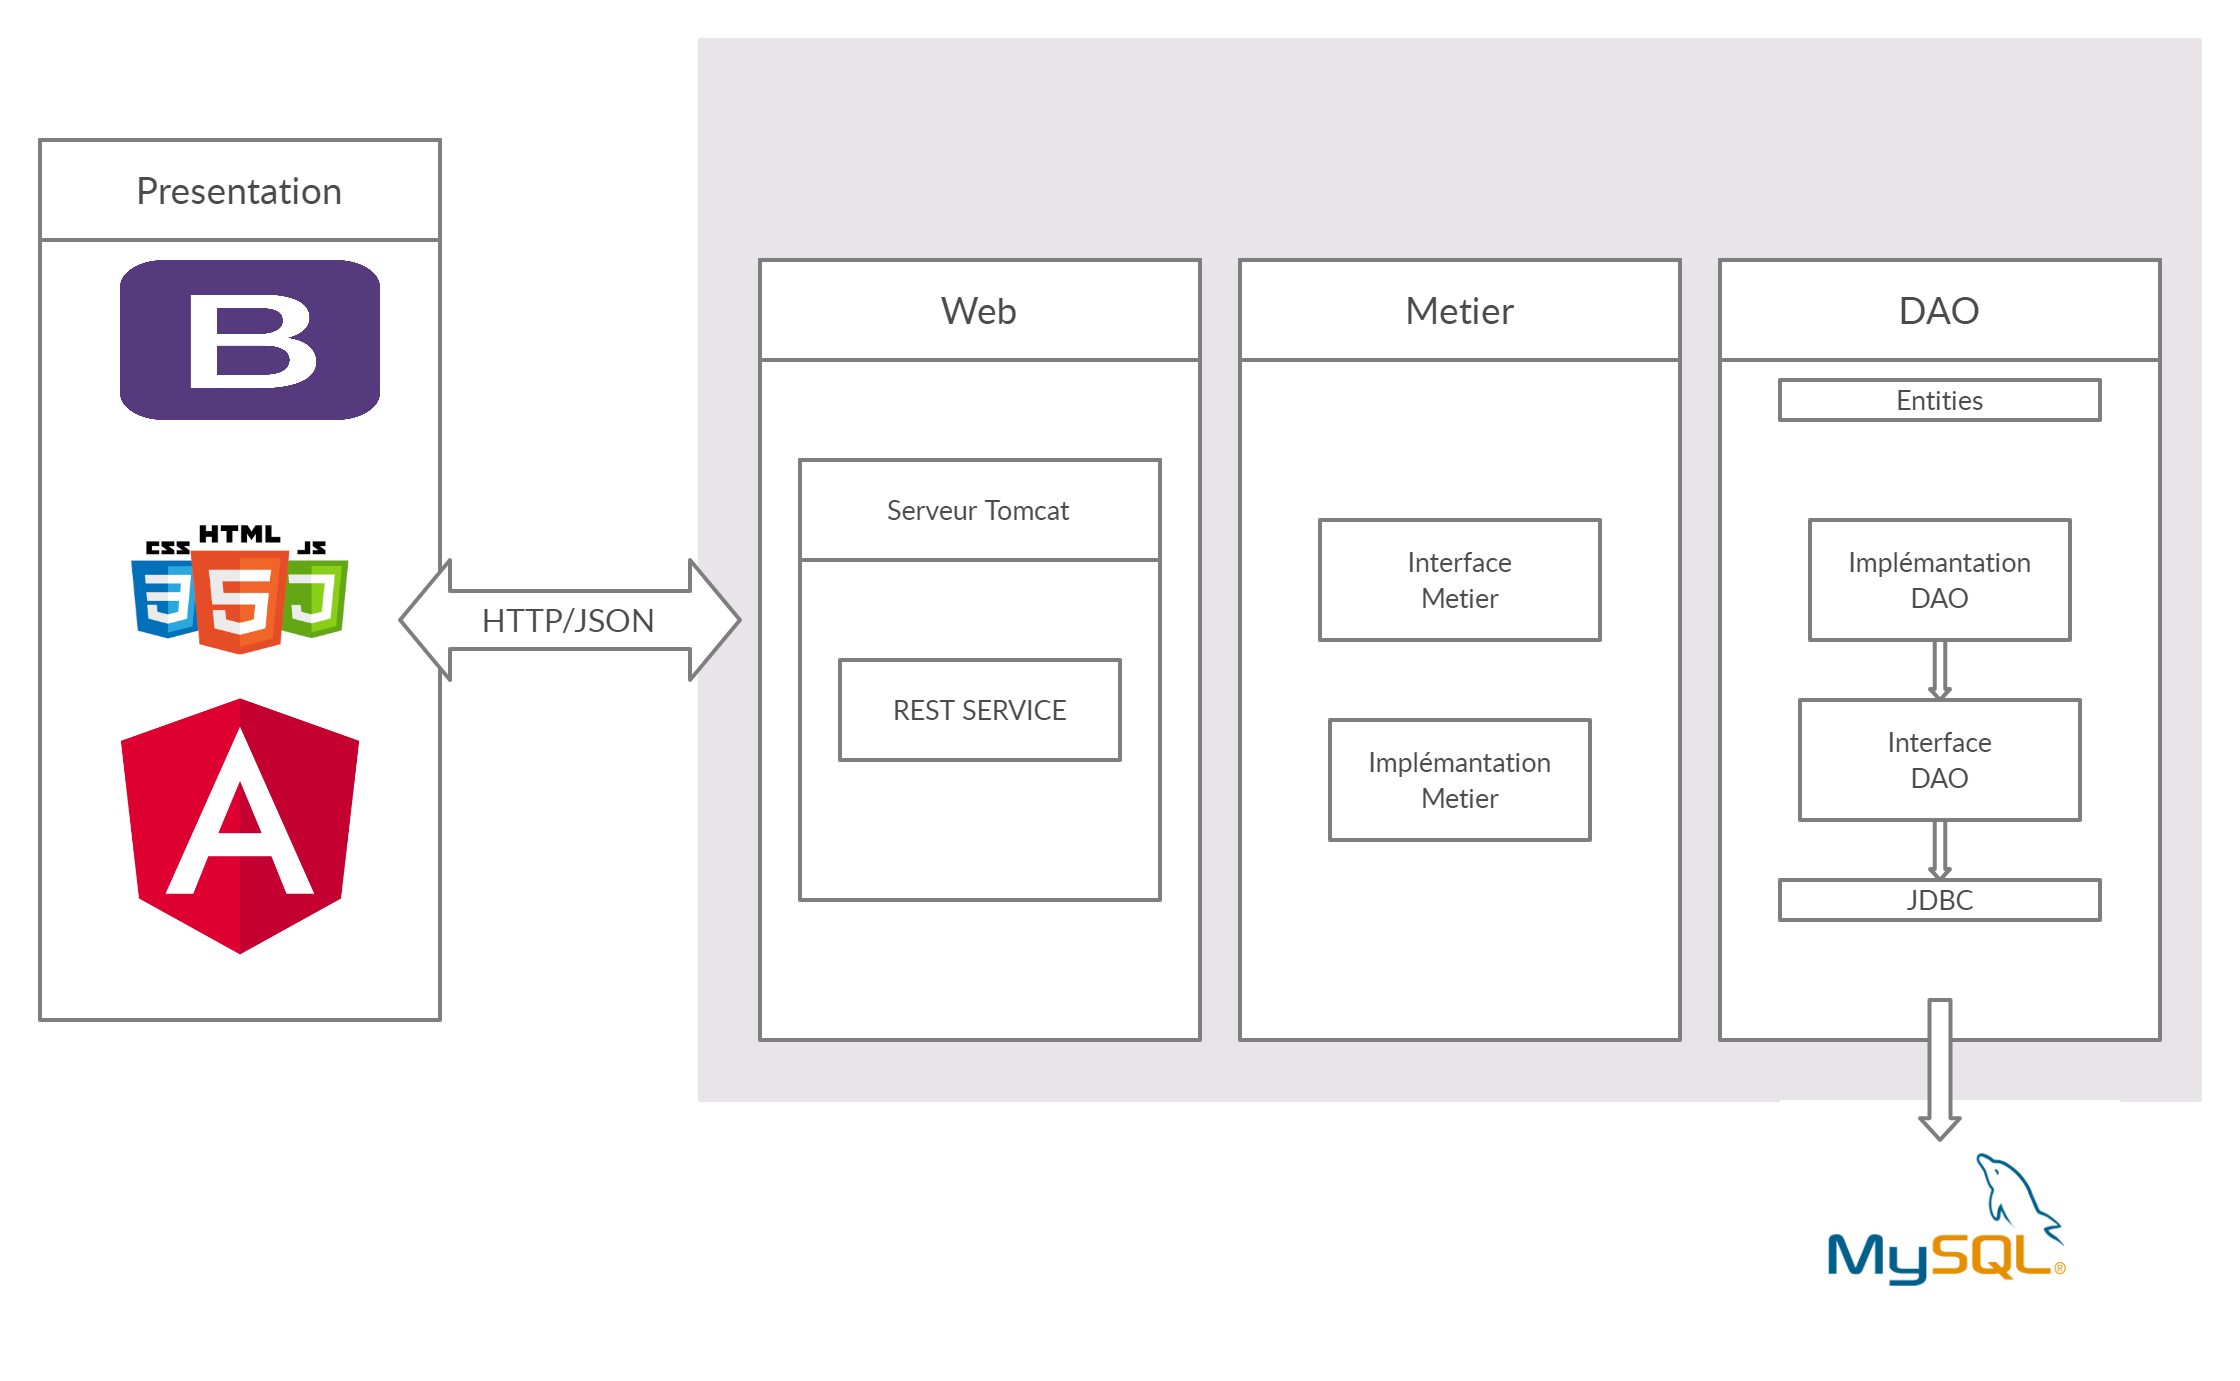
\includegraphics[width=17cm]{archit.png}
\caption{Modèle de l’architecture de l’application}
\end{center}
\end{figure}
\noindent\textbf{Couche présentation (Client)} : correspond à la partie de l’application visible et
interactive avec les utilisateurs. Elle communique avec la couche métier par les web services
et le protocole HTTP.\\
\textbf{Couche métier (Business Layer)} : correspond à la partie fonctionnelle de l’application responsable de l’implémentation de la « logique ». Celle-ci décrit les opérations que
l’application opère sur les données en fonction des requêtes des utilisateurs, effectuées au
travers de la couche présentation.\\
\textbf{Couche accès aux données (Data Layer)} : chargée de l’accès aux données et de
leur manipulation.\\
\subsection{Diagramme de classe}
Dans ce qui suit, une présentation du diagramme de classe de l’application. Ce diagramme représente le noyau du système et de tous les traitements métiers liés au projet.


\begin{figure}[!h]
\begin{center}
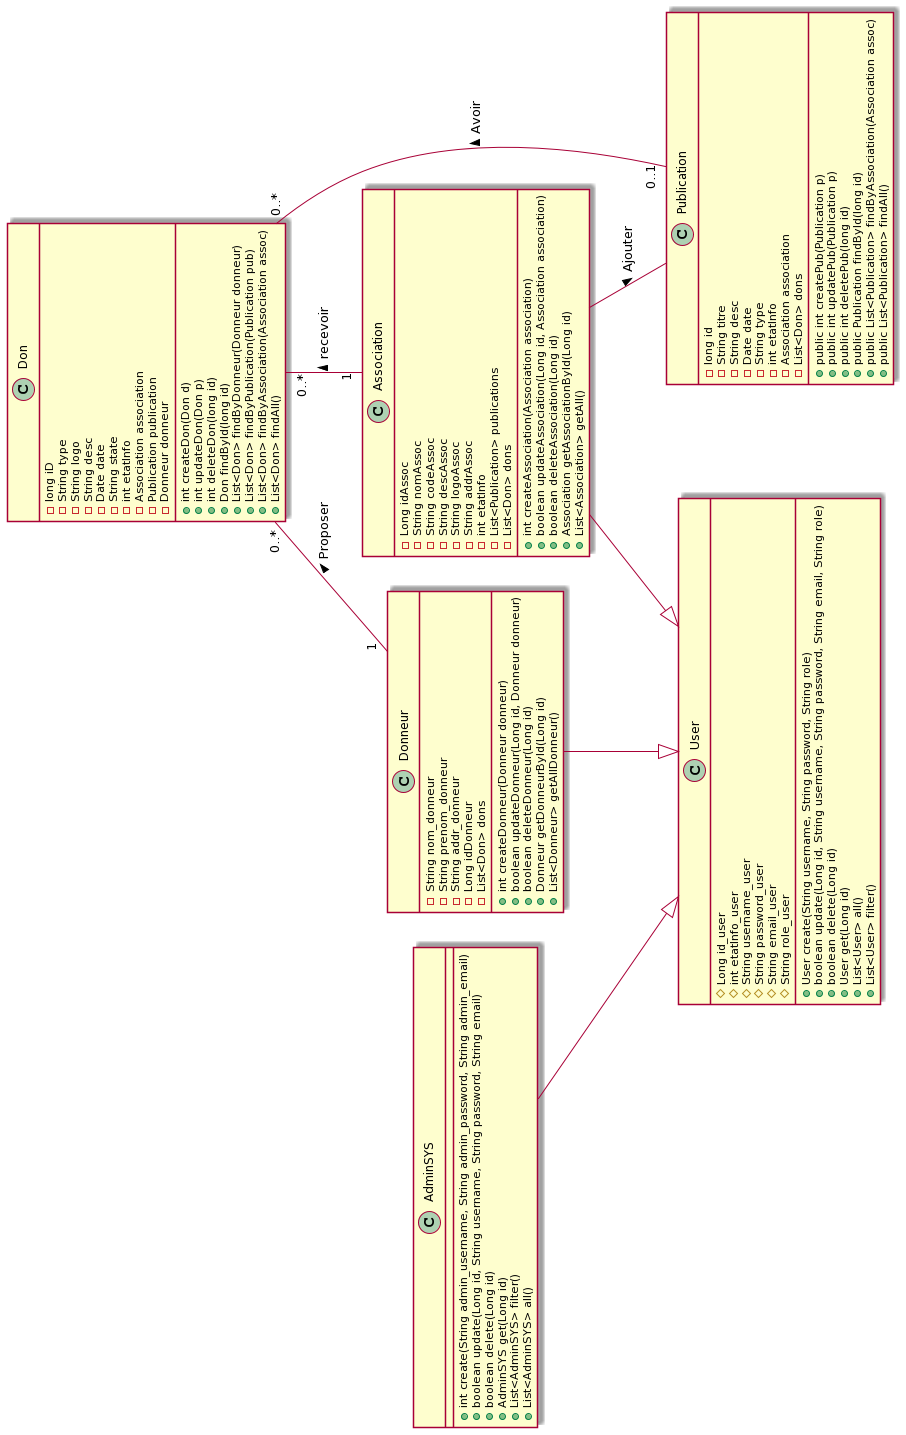
\includegraphics[width=14cm]{DCL.png}
\caption{Diagramme de classe}
\end{center}
\end{figure}
\chapter{Realisation}
Nous allons présenter dans cette partie quelques interfaces des l’application réalisée.


\begin{figure}[!h]
\begin{center}
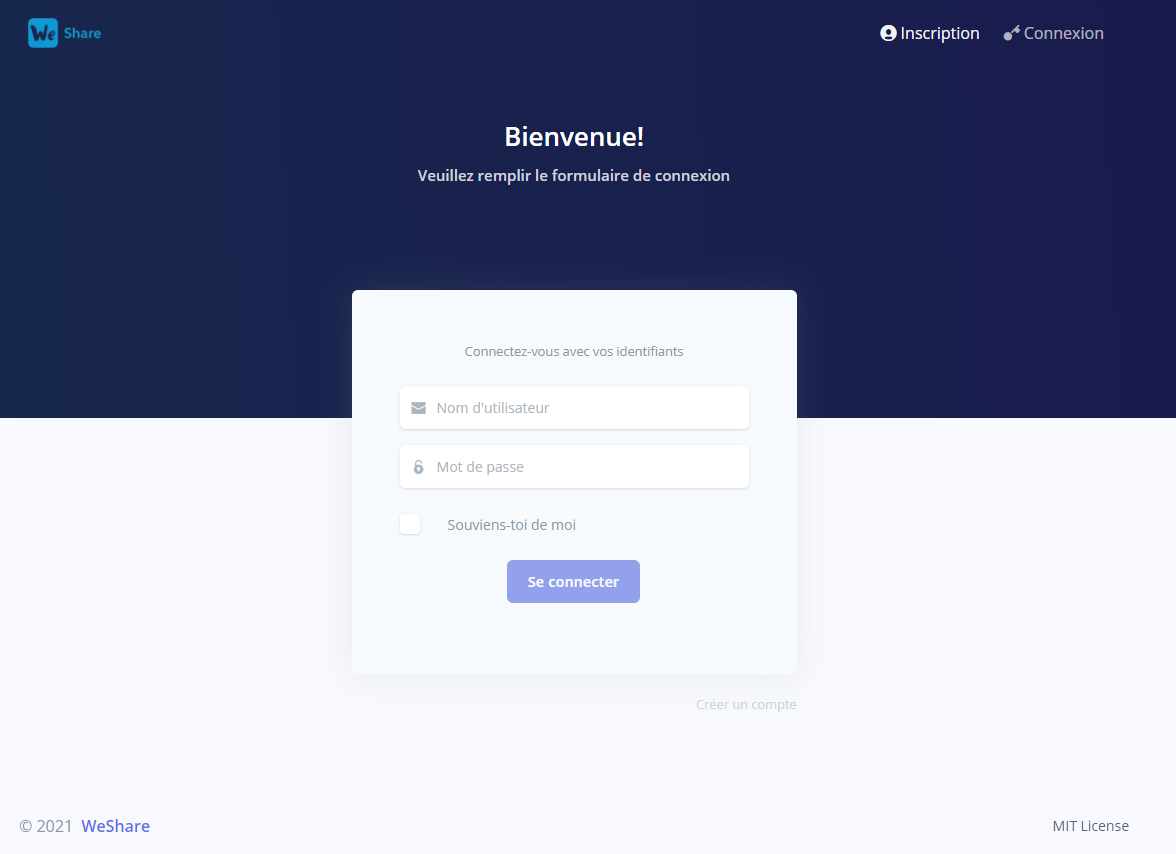
\includegraphics[width=17cm]{Login.png}
\caption{Login}
\end{center}
\end{figure}




\begin{figure}[!h]
\begin{center}
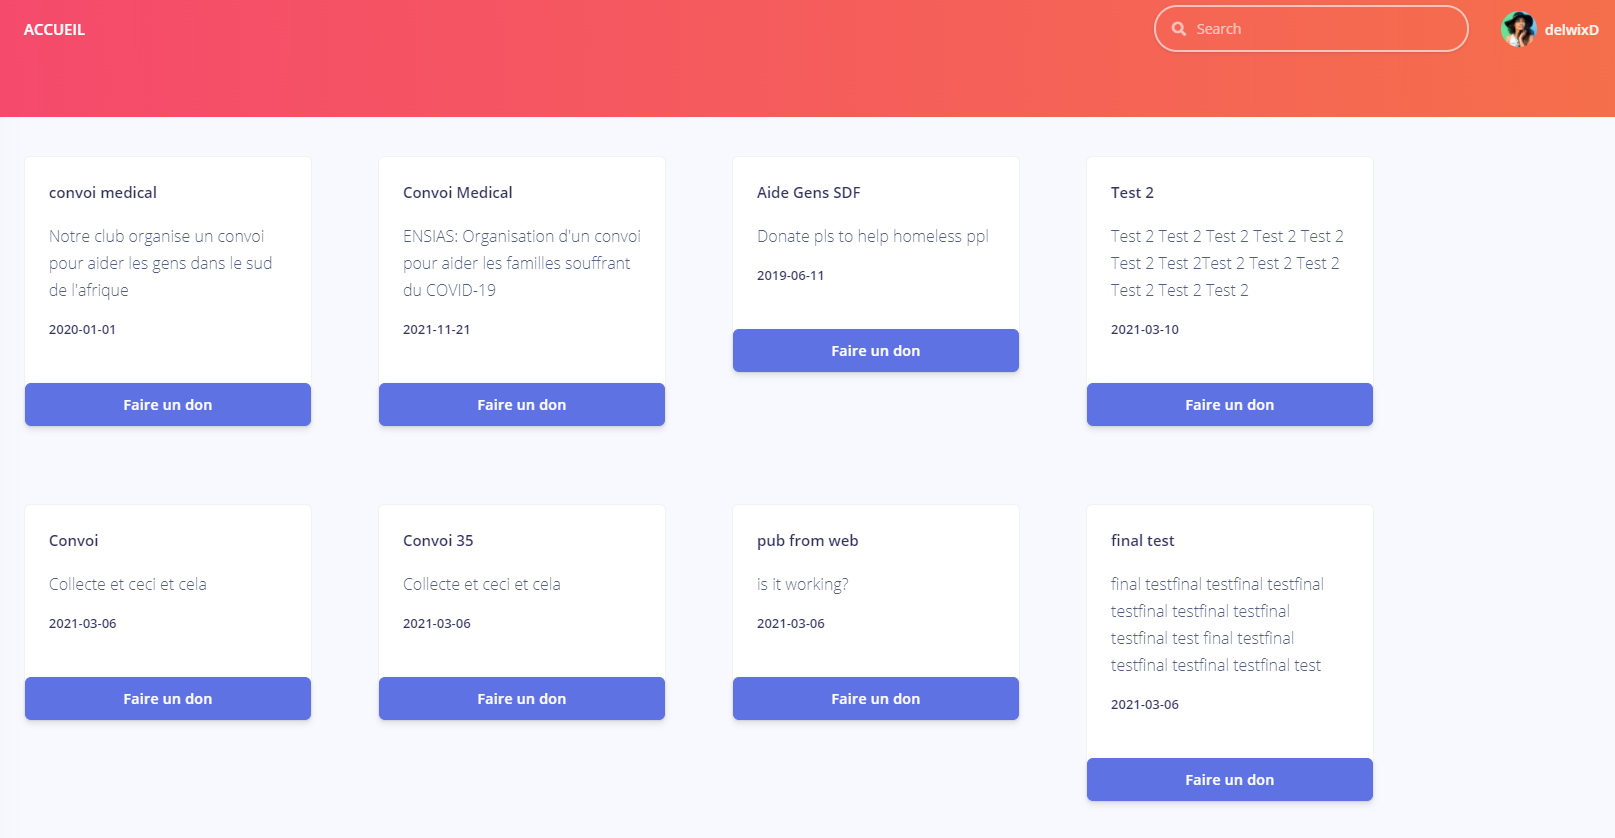
\includegraphics[width=17cm]{Acceuil.png}
\caption{Acceuil}
\end{center}
\end{figure}


\begin{figure}[!h]
\begin{center}
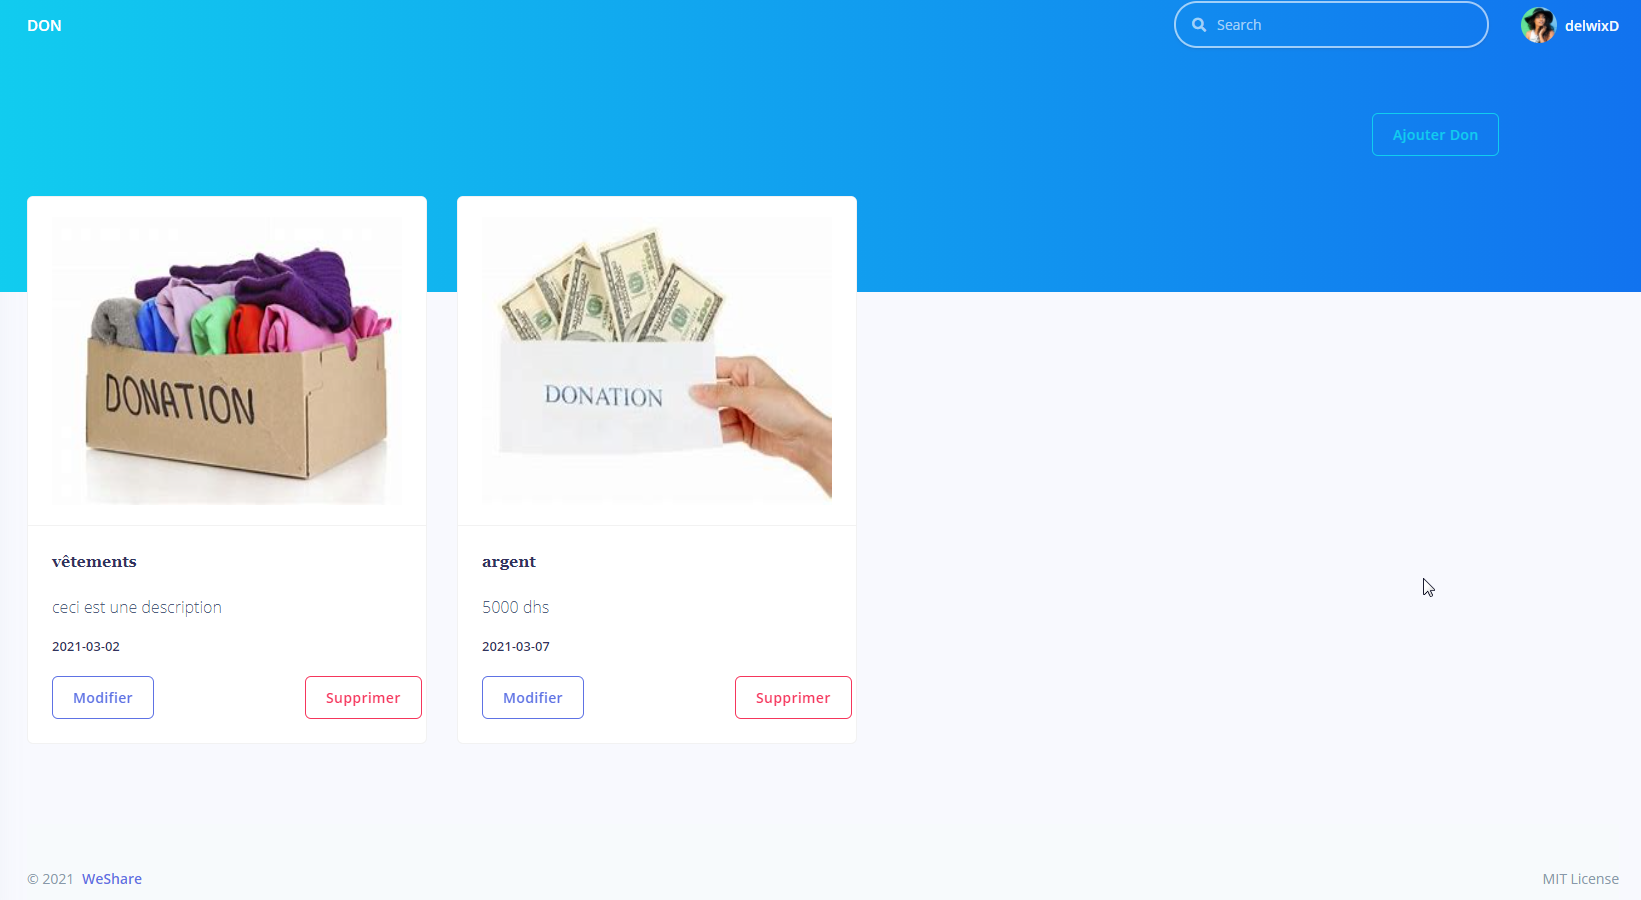
\includegraphics[width=17cm]{dons.png}
\caption{Liste des dons d'un utilisateur}
\end{center}
\end{figure}


\begin{figure}[!h]
\begin{center}
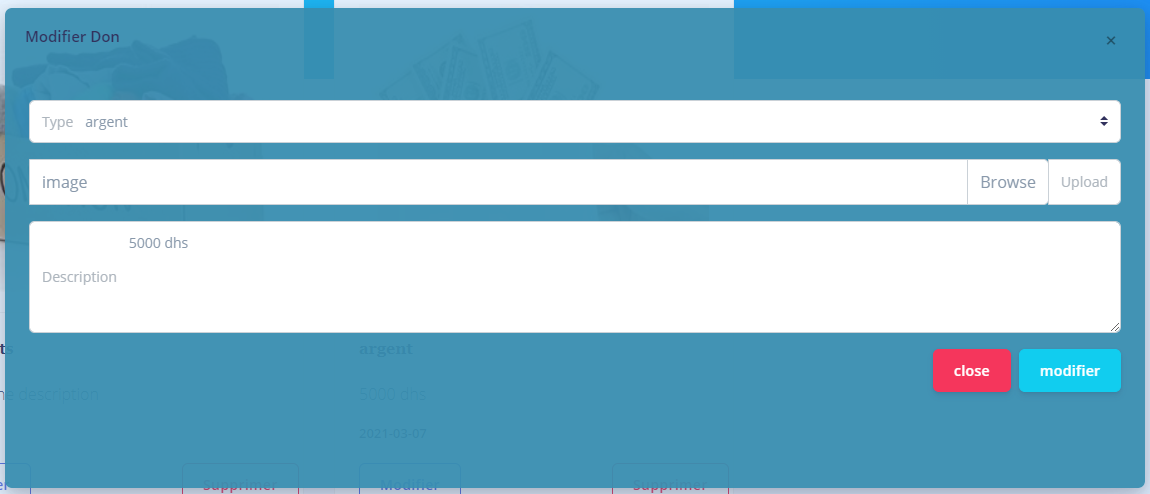
\includegraphics[width=17cm]{modification don.png}
\caption{Interface de modification d'un don}
\end{center}
\end{figure}

\begin{figure}[!h]
\begin{center}
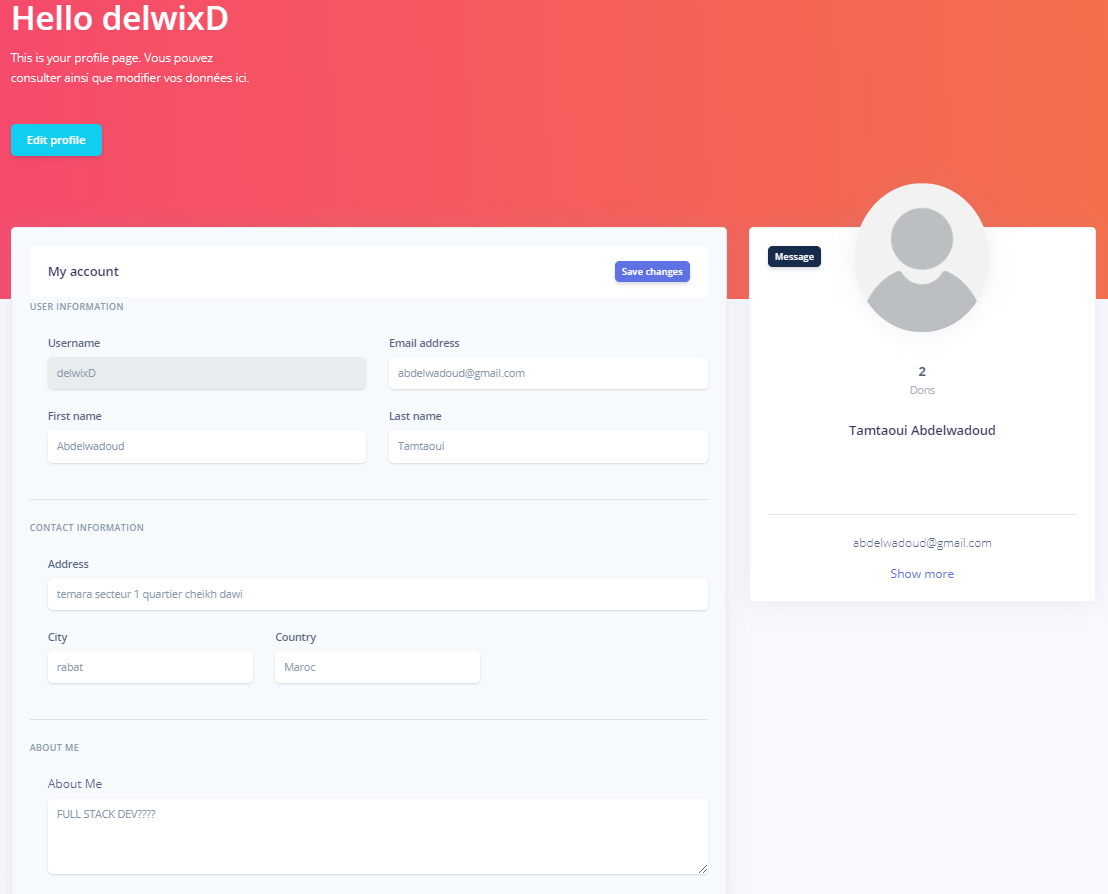
\includegraphics[width=17cm]{profile3Donneur.png}
\caption{Page Profile d'un donneur}
\end{center}
\end{figure}


\begin{figure}[!h]
\begin{center}

\includegraphics[width=7cm]{Association menu.png}
\caption{Barre menu d'une association}
\end{center}
\end{figure}

\begin{figure}[!h]
\begin{center}
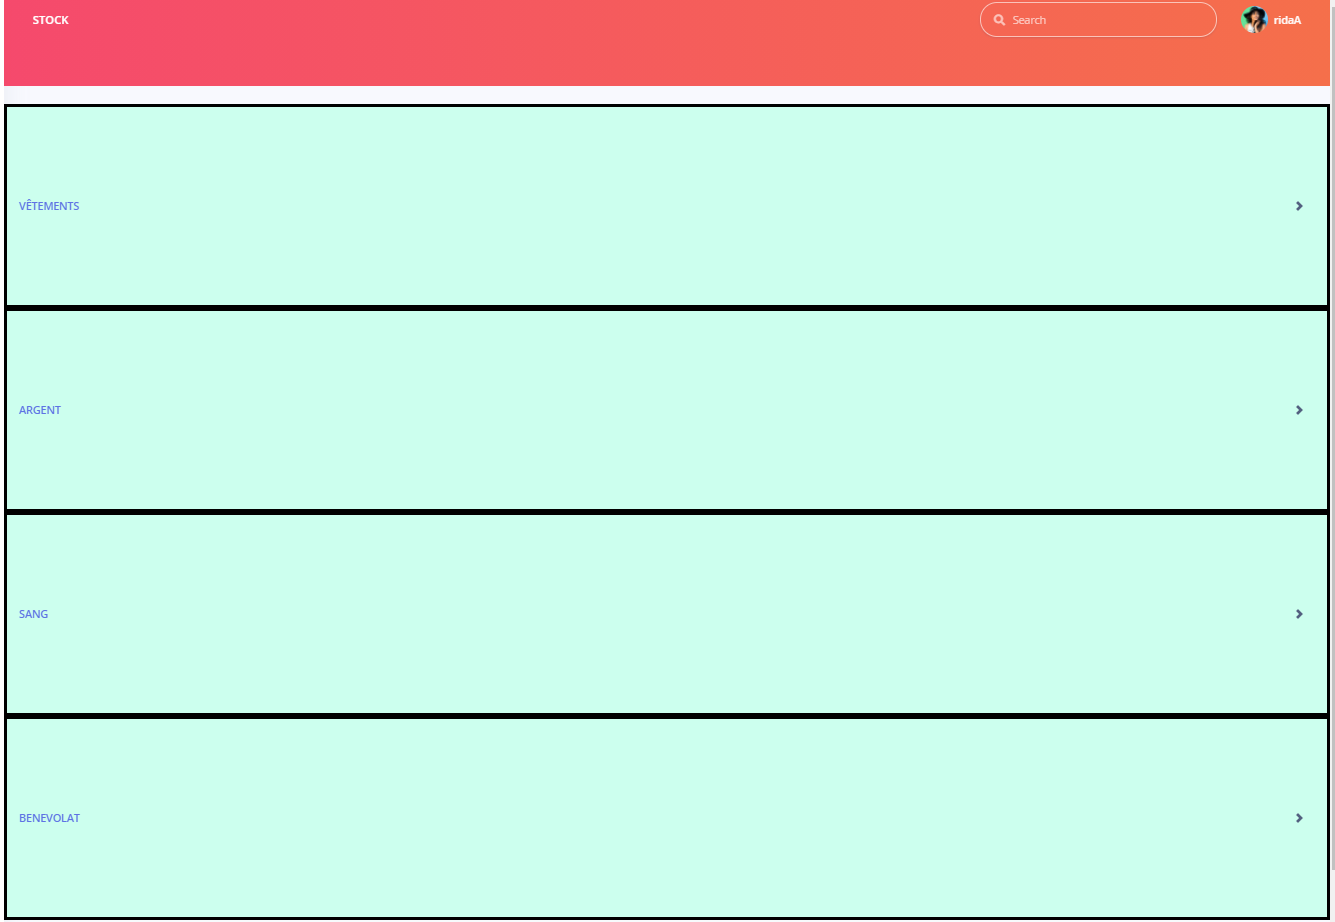
\includegraphics[width=17cm]{stock.png}
\caption{Stock d'une association}
\end{center}
\end{figure}

\begin{figure}[!h]
\begin{center}
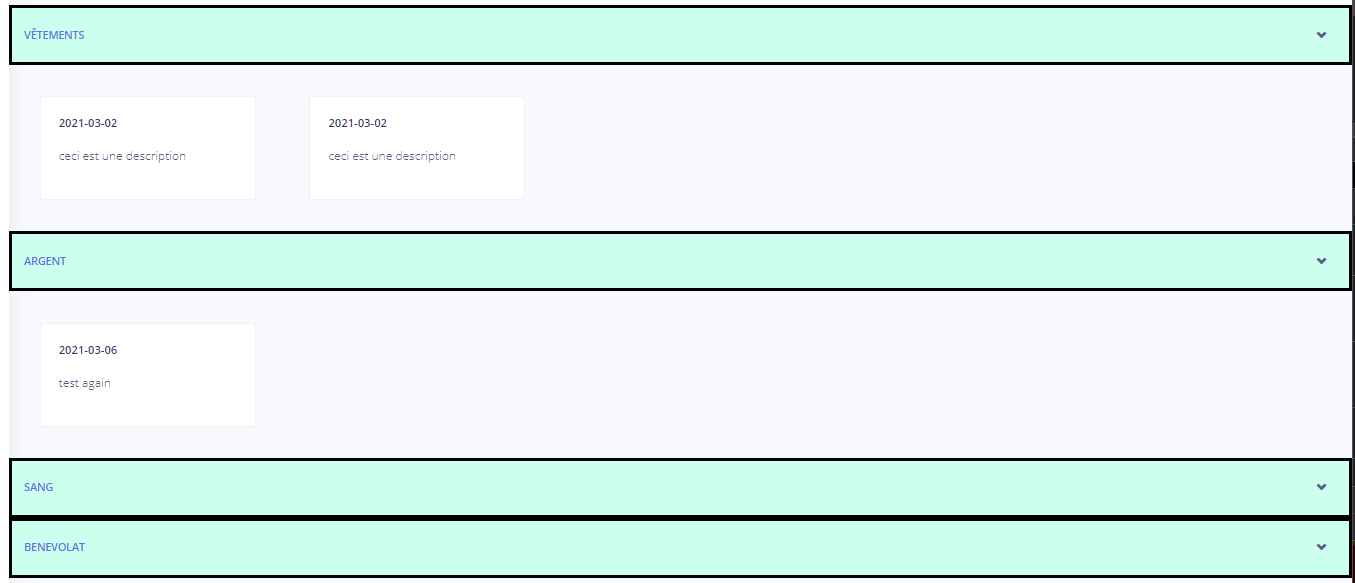
\includegraphics[width=17cm]{stock2.png}
\caption{Stock d'une association}
\end{center}
\end{figure}


\begin{figure}[!h]
\begin{center}
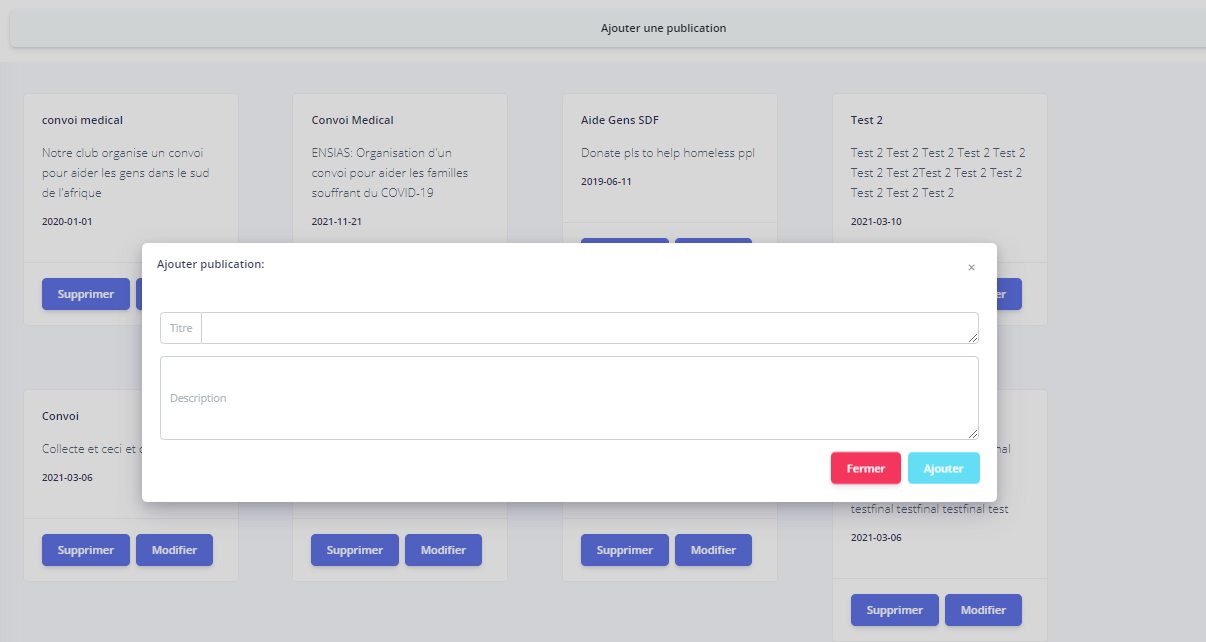
\includegraphics[width=17cm]{ajout Pub.png}
\caption{Stock d'une association}
\end{center}
\end{figure}